\section{Descriptive Analysis}
\label{sec:descriptive_analysis}

We split our descriptive analysis into two parts.
First, we analyze the trips in different forms, such as demand, availability and
idle time along multiple spatial and temporal resolutions. Then we analyze the
relationships between trips and other influencing factors, such as weather,
land use and points of interests.


\subsection{Spatial And Temporal Analysis Of Trips}
\label{subsec:descriptive_analysis_spatial_temporal}

In order to get a better understanding on where possible hot spots of bicycle
demand and availability in the system are, we create and investigate choropleth maps,
where we aggregate demand and availability by h3 hexagons.
First we plot the total flow of bicycles, that is the sum of all incoming and
outgoing trips. This can help us to identify hot spots.

\begin{figure}[htb]
    \centering
    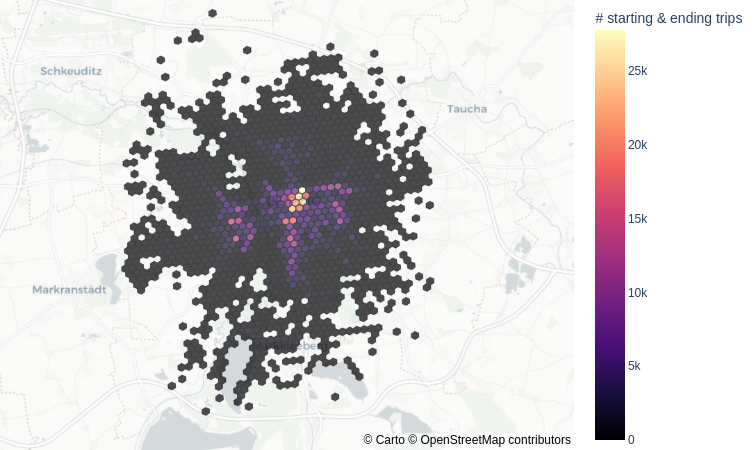
\includegraphics[width=0.8\textwidth]{Figures/descriptive_analysis/total_flow.png}
    \caption{Total Flow Of Bicycles Per Hexagon}
    \label{fig:descriptive_analysis_total_flow}
\end{figure}

With the plot as seen in figure \ref{fig:descriptive_analysis_total_flow} we
can already hots pots in the center of city, where the train station as well as
the most shopping areas are, as well as a cluster of high flow hexagons in the
west and east of the city, where residential areas are.
We also see that the the hexagons around the borders of the city have very low flow.
This shows that it is possible to satisfy a large portion of the demand by just focusing on the hot spots, which is an important consideration when entering the shared mobility market.

Next, we will analyze the net flow of bicycles per hexagon, which is the
difference between incoming and outgoing trips. This measure is highly relevant
for vehicle sharing system operators, as it shows imbalances in the system.
Imbalances occur when the number of trips that end are less or more than the
number of trips that start in a certain hexagon. This can lead to unmet demand
and therefore inefficient usage of resources. The result of such an analysis
can be used to perform effective relocations.

\begin{figure}[htb]
    \centering
    \begin{subfigure}[b]{0.45\textwidth}
        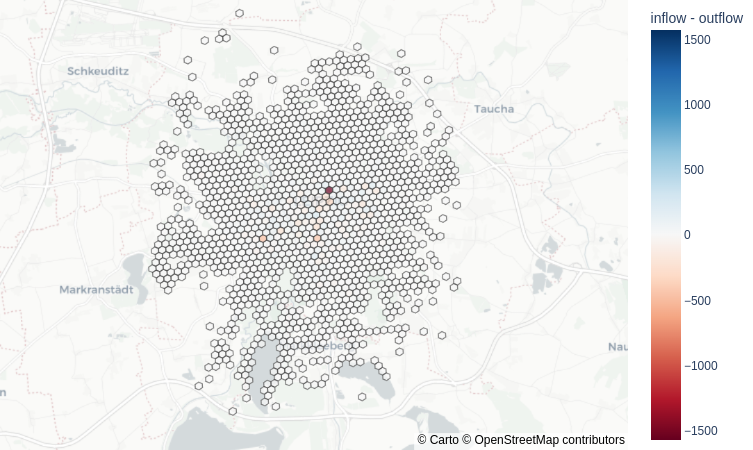
\includegraphics[width=1\textwidth]{Figures/descriptive_analysis/net_flow_original.png}
        \caption{Original Scale}
        \label{fig:descriptive_analysis_net_flow_original}
    \end{subfigure}
    \begin{subfigure}[b]{0.45\textwidth}
        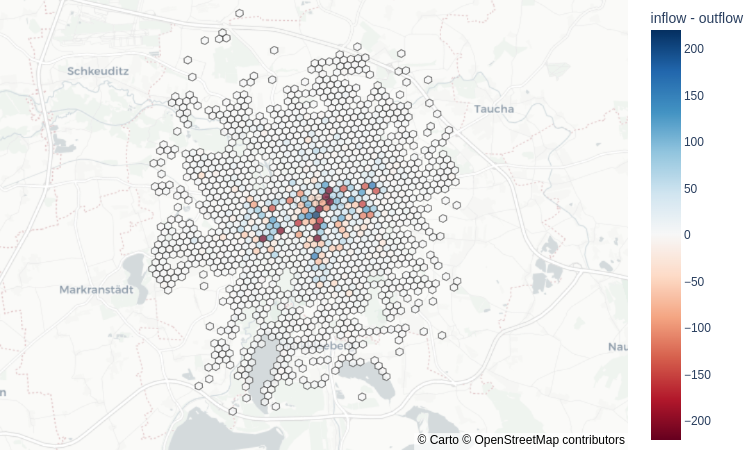
\includegraphics[width=1\textwidth]{Figures/descriptive_analysis/net_flow_rescaled.png}
        \caption{Adapted Scale}
        \label{fig:descriptive_analysis_net_flow_rescaled}
    \end{subfigure}
    \caption{Net Flow Of Bicycles Per Hexagon}
    \label{fig:descriptive_analysis_net_flow}
\end{figure}

Figure \ref{fig:descriptive_analysis_net_flow_original} shows the net flow of
bicycles per hexagon. Wee see that the net flow for the hexagon next to the
main train station is a large negative number, which means that more trips
start than end there. Our custom should expect to observe the same behaviour
when entering the market and therefore should consider to relocate bicycles
to that hexagon, in order to avoid unmet demand.
As the net flow for main train station hexagon is so large, the color scale is
so wide that we can barely see any other imbalances.
Therefore, we adjust the color scale to also see smaller imbalances.

With the adjusted color scale as seen in figure
\ref{fig:descriptive_analysis_net_flow_rescaled} we see more imbalances,
especially in the center of the city.

For an ongoing analysis of similar net flow plots, we advise to be careful with lowering the h3 resolution.
If two neighboring hexagons have negative and positive net flow, then they could cancel each other out when the resolution is decreased.
Event though a lower resolution might make it easier to understand the displayed information, it can also hide important information.

We also created an interactive plot that shows the net flows per hexagon for each month.
This plot allows us to identify seasonal imbalances, which can be further utilized to improve operational decisions.

\begin{figure}[htb]
    \centering
    \begin{subfigure}[b]{0.45\textwidth}
        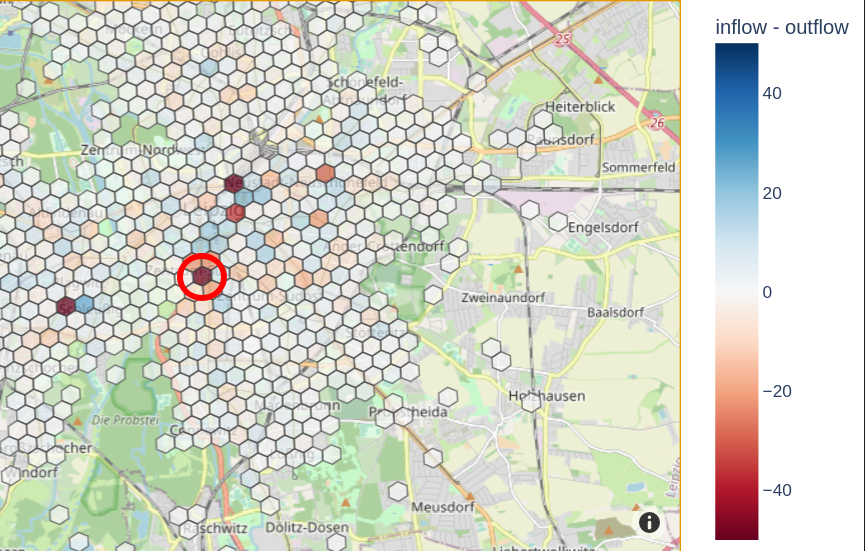
\includegraphics[width=1\textwidth]{Figures/descriptive_analysis/flossplatz_april.png}
        \caption{April}
        \label{fig:descriptive_analysis_flossplatz_april}
    \end{subfigure}
    \begin{subfigure}[b]{0.45\textwidth}
        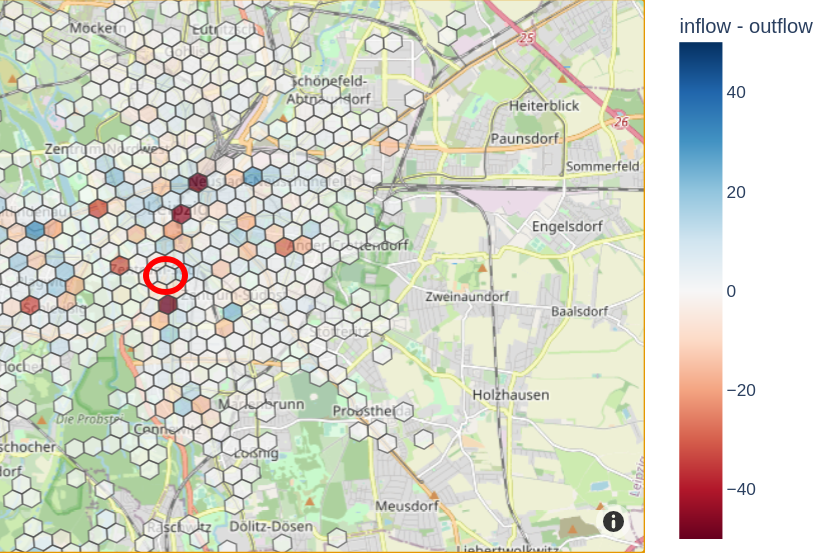
\includegraphics[width=1\textwidth]{Figures/descriptive_analysis/flossplatz_october.png}
        \caption{October}
        \label{fig:descriptive_analysis_flossplatz_october}
    \end{subfigure}
    \caption{Net Flow Of 'Floosplatz' Hexagon}
    \label{fig:descriptive_analysis_flossplatz}
\end{figure}

One such example of a seasonal imbalance can be seen in Figure \ref{fig:descriptive_analysis_flossplatz}.


Next we will analyze the idle time of bicycles. The idle time is the time
between two consecutive trips with the same bicycle. It is an important measure
for the bicycle sharing system operator as it might indicate and oversaturation
of demand. Also unusual high idle times of single bicycles can be a sign of
anomalies in the system, such as damaged or hidden bicycles.


Figure \ref{fig:descriptive_analysis_idle_time_daily} shows the median idle time of bicycles per day.
\begin{figure}[htb]
    \centering
    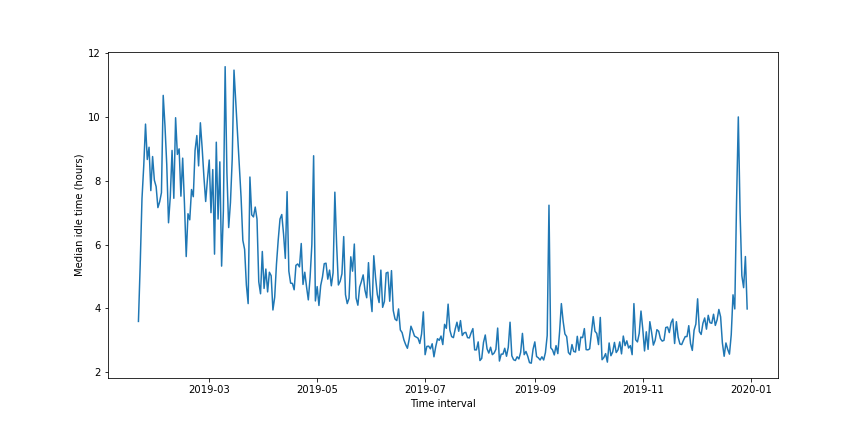
\includegraphics[width=0.8\textwidth]{Figures/descriptive_analysis/idle_time_daily.png}
    \caption{Median Idle Time Of Bicycles Per Day}
    \label{fig:descriptive_analysis_idle_time_daily}
\end{figure}

In Figure \ref{fig:descriptive_analysis_idle_time_daily} We see that the idle time of bicycles seems to decrease until around July, after which it keeps steady.
One possible explanation is that the operator was able to improve the relocation
strategy, which results in less idle time of bicycles.
Therefore, we advise the analysis of the bicycle relocations, to learn more about
NextBike's relocation strategy.

To further give concrete advise for relocations, we plot the median idle time
of bicycles per hexagon to identify critical regions with high idle times.

\begin{figure}[htb]
    \centering
    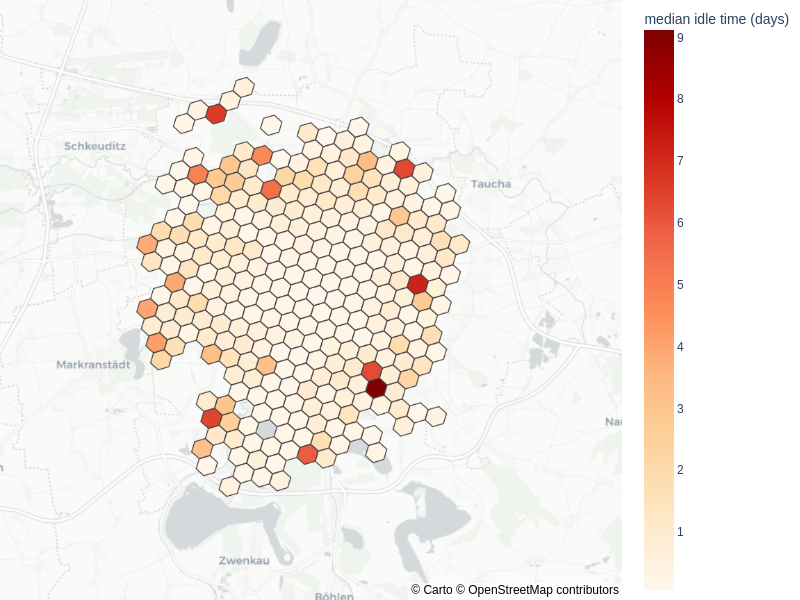
\includegraphics[width=0.8\textwidth]{Figures/descriptive_analysis/ide_time_hexagon.png}
    \caption{Median Idle Time Of Bicycles Per Hexagon}
    \label{fig:descriptive_analysis_idle_time_hexagon}
\end{figure}

We see a few hexagons at the border regions that have high idle times.
While it is possible that these idle times arise from the fact that there is only little demand in these regions, it could also be due to an increased probability of vandalism, which is not unusual in vehicle sharing systems.
We advise to carefully monitor such high idle time regions to prevent high costs through damaged vehicles.
For this sake we also provide an interactive map of the median idle time per hexagon for each month in our notebooks.

Lastly, we will also analyze the availability of bicycles. The availability,
similar to identifying hot spots and imbalances, can help to identify regions
with over saturated or under saturated demand and is therefore important for
optimization of the system.


\begin{figure}[htb]
    \centering
    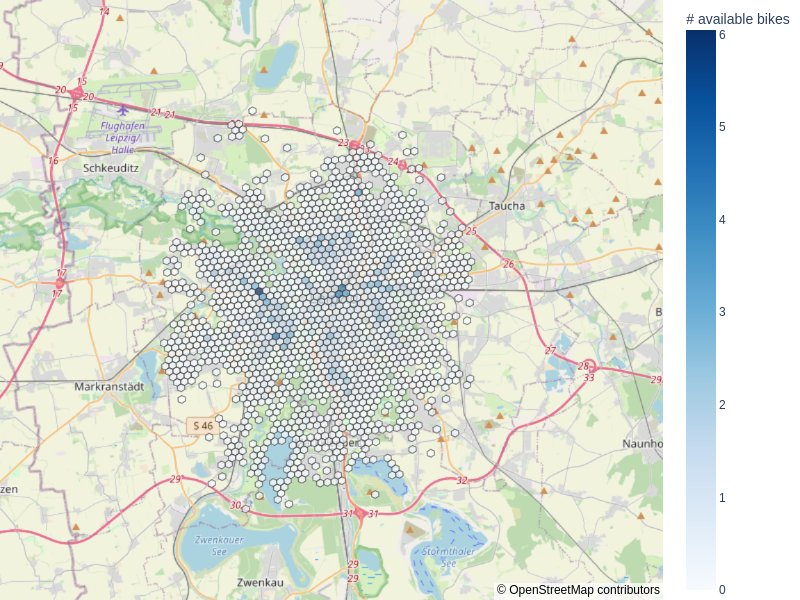
\includegraphics[width=0.8\textwidth]{Figures/descriptive_analysis/availability_per_hexagon.png}
    \caption{Availability Per Hexagon}
    \label{fig:descriptive_analysis_availability_per_hexagon}
\end{figure}

We see a few hexagon with high availability, three of them are around the main
train station, but the one with the highest availability is in the west. To
understand the cause for this increased availability better we reviewed our
land use data for this specific hexagon and found that the hexagon mostly
consists of "continous urban fabric". Looking at the area with Google Street
View also revealed that the area mostly consists of residential buildings.
Eventhough, we would expect a hexagon with high availability to have a higher
inflow than outflow and/or a higher idle time of bicycles, we do not see any
evidence for this. Therefore the high availability has to be caused by a constant,
regular and balanced inflow and outflow of bicycles, which is very good in
terms of efficiency. It might be that people living in the area around often
use bicycles to get to work and back, which would result in a balanced flow.


\subsection{Relationships Between Trips And Other Influencing Factors}
\label{subsec:descriptive_analysis_relationships}
